\documentclass{article}
\usepackage{zpj}
\usepackage{tikz}
\newcommand{\comm}[1]{\ {\color{blue} \texttt{#1}}\ }
\begin{document}
\title{Energy of Electrostatic Field in a Triangle}
\author{\zpj}
\maketitle
\section{Energy of a triangle}
For a triangle $ABC$, assume the points have potential $\varphi_a,\varphi_b,\varphi_c$. As shown in Fig.~\ref{nab}, $AB'\perp AC, AC'\perp AB$, combine the components of $\nabla\varphi$, we have
\[(\nabla\varphi)^2=\frac{1}{\sin^2 A}\left(\frac{\varphi_{ab}^2}{c^2}+\frac{\varphi_{ac}^2}{b^2}-\frac{2\varphi_{ab}\varphi_{ac}\cos A}{bc}\right)\]
\begin{figure}[htbp]
\centering
 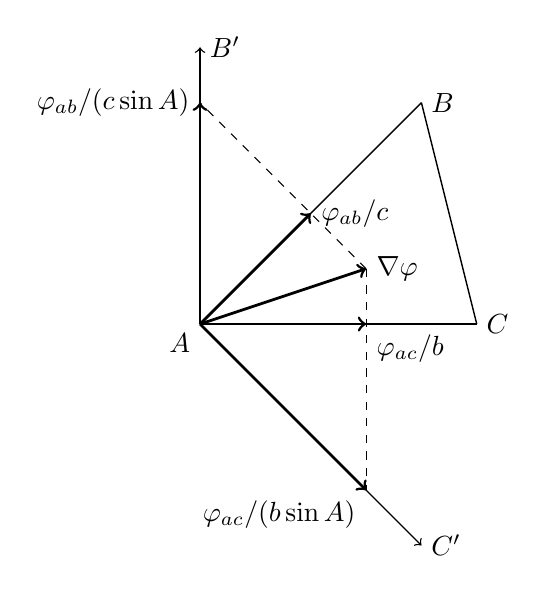
\begin{tikzpicture}
\pgfsetxvec{\pgfpoint{20pt}{0}}
\pgfsetyvec{\pgfpoint{0}{20pt}}
  \draw[->,line width=0.5pt] (0,0)node[below left]{$A$}--(4,-4)node[right]{$C'$};
  \draw[line width=0.5pt] (0,0)--(5,0)node[right]{$C$};
  \draw[line width=0.5pt] (4,4)node[right]{$B$}--(5,0);
  \draw[line width=0.5pt] (0,0)--(4,4);
  \draw[->,line width=0.5pt] (0,0)--(0,5)node[right]{$B'$};
  \draw[dashed] (3,1)--(0,4);
  \draw[dashed] (3,1)--(3,-3);
  \draw[->,line width=1pt] (0,0)--(2,2)node[right]{$\varphi_{ab}/c$};
  \draw[->,line width=1pt] (0,0)--(3,-3)node[below left]{$\varphi_{ac}/(b\sin A)$};
  \draw[->,line width=1pt] (0,0)--(0,4)node[left]{$\varphi_{ab}/(c\sin A)$};
  \draw[->,line width=1pt] (0,0)--(3,0)node[below right]{$\varphi_{ac}/b$};
  \draw[->,line width=1pt] (0,0)--(3,1)node[right]{$\nabla\varphi$};
 \end{tikzpicture}
 \caption{Using contra-variant bases to evaluate $(\nabla\varphi)^2$}\label{nab}
\end{figure}

The area of triangle is
\[S=\frac{bc\sin A}{2}\]

The energy of this triangle is
\begin{align}
 E_{\triangle}&\propto S(\nabla\varphi)^2\\
 &\propto \frac{bc}{\sin A}\left(\frac{\varphi_{ab}^2}{c^2}+\frac{\varphi_{ac}^2}{b^2}-\frac{2\varphi_{ab}\varphi_{ac}\cos A}{bc}\right)
\end{align}
对$\varphi_a$求导得到:
\begin{equation}
 \frac{\pp E_\triangle}{\pp \varphi_a}\propto \left(\frac{b}{c\sin A}-\cot A\right)\varphi_{ab}+\left(\frac{c}{b\sin A}-\cot A\right)\varphi_{ac}\label{a}
\end{equation}
其中:
\[\frac{b}{c\sin A}-\cot A=\frac{b-c\cos A}{c\sin A}=\frac{a\cos C}{a\sin C}=\cot C\]
同理\[\frac{c}{b\sin A}-\cot A=\cot B\]
故\ref{a}化为
\begin{equation}
 \frac{\pp E_\triangle}{\pp \varphi_a}\propto \varphi_{ab}\cot C+\varphi_{ac}\cot B
 \label{comp}
\end{equation}
\section{Stationary point equation for energy minimum}
Let $E$ be the total energy and use $i$ to mark all triangles containing $A$. $B_i, C_i$ are other points in triangle $i$. In the stationary point, we have
\[ \frac{\pp E}{\pp \varphi_a}=\sum_i\frac{\pp  E_i}{\pp \varphi_a}
 \propto\sum_i \varphi_{ab_i}\cot C_i+\varphi_{ac_i}\cot B_i=0\]
So,
\[\sum_i\left(\cot C_i+\cot B_i\right)\varphi_{a}=\sum_i\left(  \varphi_{b_i}\cot C_i+\varphi_{c_i}\cot B_i\right) \]

\[\Rightarrow\varphi_a=\frac{\sum_i \varphi_{b_i}\cot C_i+\varphi_{c_i}\cot B_i}{\sum_i\cot C_i+\cot B_i}
\]

Assume we know coordinates of a triangle $ABC$. To calculate $\cot A$, we define $\bm b=\overrightarrow{AB}, \bm c=\overrightarrow{AC}$. 
\[ \cot A=\frac{bc\cos A}{bc\sin A}=\frac{\bm{b\cdot c}}{|\bm{b\times c}|}=\frac{\bm{b\cdot c}}{2S}\]

The denominator $2S$ is the same for a triangle.
\end{document}
